    % Copyright 2004 by Till Tantau <tantau@users.sourceforge.net>.
%
% In principle, this file can be redistributed and/or modified under
% the terms of the GNU Public License, version 2.
%
% However, this file is supposed to be a template to be modified
% for your own needs. For this reason, if you use this file as a
% template and not specifically distribute it as part of a another
% package/program, I grant the extra permission to freely copy and
% modify this file as you see fit and even to delete this copyright
% notice. 

\documentclass{beamer}

% There are many different themes available for Beamer. A comprehensive
% list with examples is given here:
% http://deic.uab.es/~iblanes/beamer_gallery/index_by_theme.html
% You can uncomment the themes below if you would like to use a different
% one:
%\usetheme{AnnArbor}
%\usetheme{Antibes}
%\usetheme{Bergen}
%\usetheme{Berkeley}
%\usetheme{Berlin}
%\usetheme{Boadilla}
%\usetheme{boxes}
%\usetheme{CambridgeUS}
%\usetheme{Copenhagen}
%\usetheme{Darmstadt}
%\usetheme{default}
%\usetheme{Frankfurt}
%\usetheme{Goettingen}
%\usetheme{Hannover}
%\usetheme{Ilmenau}
%\usetheme{JuanLesPins}
%\usetheme{Luebeck}
\usetheme{Madrid}
%\usetheme{Malmoe}
%\usetheme{Marburg}
%\usetheme{Montpellier}
%\usetheme{PaloAlto}
%\usetheme{Pittsburgh}
%\usetheme{Rochester}
%\usetheme{Singapore}
%\usetheme{Szeged}
%\usetheme{Warsaw}

\usepackage{kotex}
\usepackage{braket}
\usepackage{array}
\usepackage{calc}
\usepackage{datetime}
\usepackage{dsfont}
\usepackage{amsmath}
\usepackage{listings}


\title{Lecture 6.5 : Gradient Descent의 상세 }

% A subtitle is optional and this may be deleted
\subtitle{Fastcampus Math Camp}

\author{신승우}
% - Give the names in the same order as the appear in the paper.
% - Use the \inst{?} command only if the authors have different
%   affiliation.

% \institute[Universities of Somewhere and Elsewhere] % (optional, but mostly needed)
% {
  % \inst{1}%
  % Department of Computer Science\\
  % University of Somewhere
  % \and
  % \inst{2}%
  % Department of Theoretical Philosophy\\
  % University of Elsewhere}
% - Use the \inst command only if there are several affiliations.
% - Keep it simple, no one is interested in your street address.

% - Either use conference name or its abbreviation.
% - Not really informative to the audience, more for people (including
%   yourself) who are reading the slides online

\subject{Theoretical Computer Science}

% This is only inserted into the PDF information catalog. Can be left
% out. 

% If you have a file called "university-logo-filename.xxx", where xxx
% is a graphic format that can be processed by latex or pdflatex,
% resp., then you can add a logo as follows:

% \pgfdeclareimage[height=0.5cm]{university-logo}{university-logo-filename}
% \logo{\pgfuseimage{university-logo}}

% Delete this, if you do not want the table of contents to pop up at
% the beginning of each subsection:


% \AtBeginSection[]
% {
  % \begin{frame}<beamer>{Outline}
    % \tableofcontents[currentsection,hideallsubsections]
  % \end{frame}
% }

% Let's get started
\begin{document}

\begin{frame}
 \titlepage
\end{frame}


% \begin{frame}{선형변환의 예시 : 확대/축소} 
% 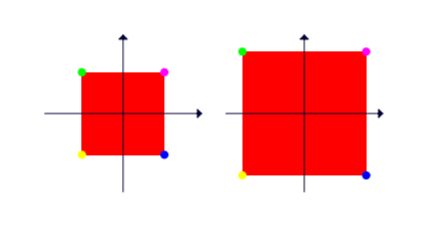
\includegraphics[width=10cm,keepaspectratio]{scale1}
% \end{frame}

% \begin{frame}{Outline}
  % \tableofcontents[hideallsubsections]
  % % You might wish to add the option [pausesections]
% \end{frame}

% Section and subsections will appear in the presentation overview
% and table of contents.



\begin{frame}{Gradient Descent : Linear Regression}
우리가 지난번에 다루었던 Linear Approximation의 경우, 다음을 만족하는 $\vec{x}$를 해석적으로 구할 수 있었다. 

\begin{equation} 
min_{\vec{x}} |A\vec{x} - \vec{b}| 
\end{equation}

이를 만약 Gradient Descent 알고리즘을 이용하여 구한다면, 대략 다음과 같은 과정을 따를 것이다. 

\begin{itemize} 
\item Loss Function $J(\theta)$를 구성한다. 여기서는 $|A\vec{x} - \vec{b}|$가 Loss Function이 될 것이며, $\theta$는 $\vec{x}$로, loss function의 값을 계산하는 파라미터일 것이다. 
\item $\nabla_{\theta} J(\theta)$를 계산한다. 
\item $\theta$의 초기값을 지정한다. 
\item 데이터를 이용해서 parameter를 조정한다. 
\end{itemize}
\end{frame}

\begin{frame}{Gradient Descent Variants}

이 때, 어떤 식으로 데이터를 이용하고 그래디언트를 구하는지에 따라서 아래의 3가지 변형이 있다. 

\begin{itemize} 
\item Batch Gradient Descent
\item Stochastic Gradient Descent 
\item Mini-Batch Gradient Descent 
\end{itemize}
\end{frame}


\begin{frame}{Batch Gradient Descent}
가장 기본적인 Gradient Descent로, 다음의 과정에 따라 최적값을 찾는다. 

\begin{itemize} 
\item 처음 parameter와 learning rate $\eta$를 정한다. 
\item 모든 데이터에 대해서 그 지점에서의 gradient descent 값을 결정한다. 
\item parameter을 $\theta_{n+1} = \theta_n - \eta \nabla_{\theta} J(\theta)$와 같이 업데이트한다. 
\end{itemize}

\end{frame}

\begin{frame}

여기서 모든 데이터를 이용한다는 것에 대해서 일견 이해하기 어려울 수 있기 때문에, 선형 회귀의 예시를 들어 설명하고자 한다. 

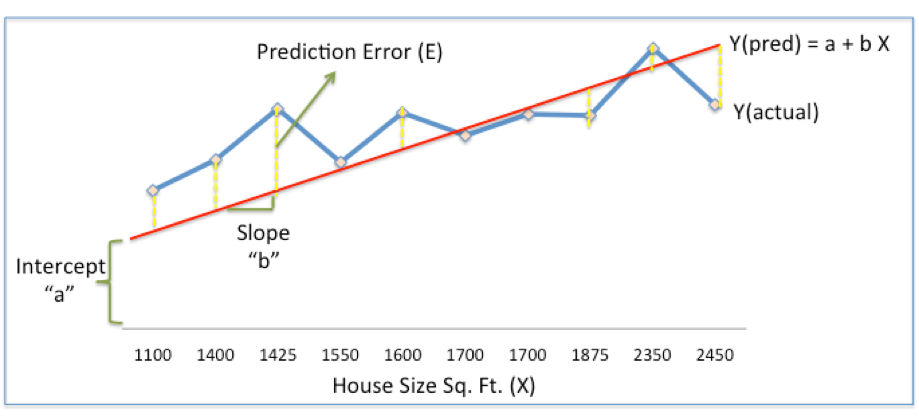
\includegraphics[width=10cm,keepaspectratio]{err}

선형 회귀에서의 parameter은 a,b 두 개이다. 이 때, 우리는 loss function을 

\begin{equation} 
\sum_i ((ax_i + b) - y_i)^2 
\end{equation}
로 정의하여, 이의 gradient를 구할 수 있다. 이 때 gradient를 구하는 과정은 단순 미분이므로 데이터를 사용하지 않는다. 이후, 저 loss function을 계산할 때 모든 데이터를 다 반영하여 계산하는 것이다. 
\end{frame}

\begin{frame}{Stochastic Gradient Descent} 
Stochastic Gradient Descent는 이와는 조금 다르다. 이 때는 각 데이터 하나에 대해서만 loss function을 계산한다. 
\begin{equation}
\theta_{n+1} = \theta_n - \eta \nabla_{\theta} J(\theta;(x_i, y_i))
\end{equation}

즉, 위 loss function과는 다르게 $\sum$이 없다. 일반적으로 stochastic gradeint descent는 탐색 과정에서 parameter 값이 크게 출렁이며, 그렇기에 학습이 진행될 때마다 learning rate를 줄여주는 추가적인 optimization을 시행하기도 한다. 
\end{frame}

\begin{frame}{Mini-batch Gradient Descent} 
Mini-bacth는 두 방법의 혼합으로, 한번에 batch size만큼의 데이터를 이용하여 optimization을 하는 것이다. 즉, loss function을 계산할 때 다음과 같이 하게 된다. 

\begin{equation} 
J(a,b) = sum_{i=k}^{k+b} ((ax_i + b) - y_i)^2 
\end{equation}

이 때 b는 batch size이다. 
\end{frame}


\begin{frame}{Challenges in Gradient Descent}
위와 같은 기본적인 Mini-batch Gradient Descent 알고리즘은 실험적으로 볼 때 항상 잘 converge 하지는 않으며, 이는 아래의 이유들에 기인한다. 

\begin{itemize} 
\item learning rate $\eta$의 선택 
\begin{itemize} 
\item learning rate를 너무 작거나 큰 고정된 값으로 선택할 경우, 각각 문제가 있다. 
\item learning rate를 학습 과정에서 바꿀 수 있도록 미리 정해놓는 경우, 학습 데이터의 특성을 반영하지 못한다. 
\item 모든 parameter들에 대해서 같은 learning rate가 반영되므로, 적절하지 못한 경우가 생긴다. 
\end{itemize}
\item Local Minima에 갇혀서 global minima로 수렴하지 못하는 경우 
\end{itemize}
\end{frame}

\begin{frame}{Various Gradient Descent Optimizations }

위 문제들을 해결하기 위하여, 아래의 다양한 optimizing strategy를 사용한다. 

\begin{itemize} 
\item Momentum 
\item Nesterov Accelerated Gradient 
\item Adagrad 
\item 등등등... 
\end{itemize}


\end{frame}

\begin{frame}{Momentum}
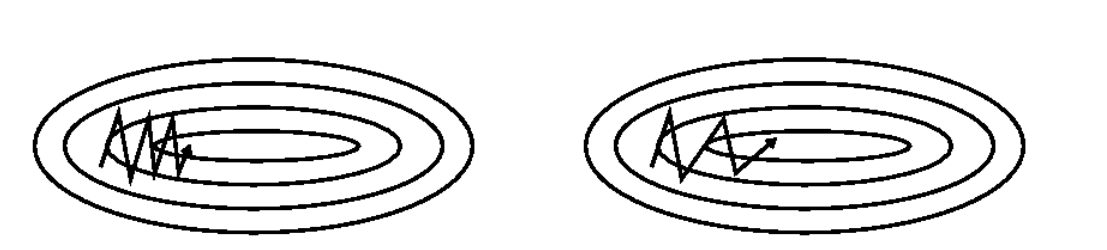
\includegraphics[width=10cm,keepaspectratio]{momentum}

일반적으로, 위에서 제시된 SGD 방법들은 어떤 특정한 한 축에 대해서 곡면에 훨씬 steep할 경우, 학습이 느려지는 경향이 있다. 따라서 다음과 같이 기존의 움직임을 반영하는 일종의 \textit{운동량} 을 추가적으로 더해준다. 

\begin{eqnarray} 
v_t &=& \gamma v_{t-1} + \eta \nabla_{\theta} J \\ 
\theta &=& \theta - v_t
\end{eqnarray} 
\end{frame}

\begin{frame}{Nesterov Momentum}
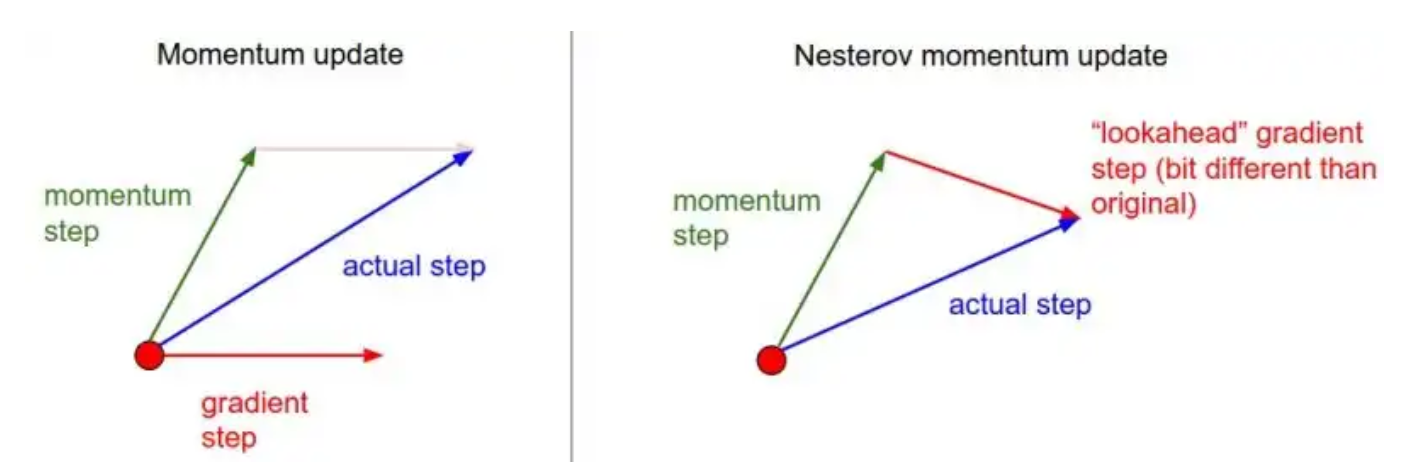
\includegraphics[width=10cm,keepaspectratio]{acc}

위 운동량을 개량한 버젼이 Nesterov Momentum이다. 이는 우리가 기존에 생각하던 momentum에 일종의 lookahead를 주는 것이다. 

\begin{eqnarray} 
v_t &=& \gamma v_{t-1} + \eta \nabla_{\theta} J(\theta-\gamma v_{t-1}) \\ 
\theta &=& \theta - v_t
\end{eqnarray} 
\end{frame}


\begin{frame}{Adagrad}

이때까지는 updating하는 방법에 대한 것이였다면, 이번에는 각 parameter에 따라서 다른 learning rate를 제공하자는 아이디어를 만든 것이다. 어떤 feature가 특정 learning rate에서 많이 바뀐다면, 그 feature에 대한 learning rate를 낮춤으로써 조금 더 안정적인 학습을 진행할 수 있으며, 반대로 거의 바뀌지 않는다면 조금 더 learning rate를 높여 더 빠른 학습을 꾀할 수 있다. 학습 과정은 다음과 같다. 

각 파라미터마다 learning rate가 다르므로, 아래 식에서는 t를 학습 횟수, i를 parameter 인덱스로 사용하겠다. 

\begin{equation} 
\theta_{t+1,i} = \theta_{t,i} - \frac{\eta}{\sqrt{G_{t, i} + \epsilon}} \nabla J(\theta_{t,i})
\end{equation} 

여기서, $G_{t, i}$는 i번째 파라미터가 t번 학습할 때까지 변한 값의 제곱의 합이며, $\epsilon$은 그저 division by zero 에러를 막기 위한 작은 값으로, 보통 $10^{-8}$ 정도의 값을 사용한다. 
\end{frame}

\begin{frame}{Adadelta}

Adagrad가 그 전의 모든 그래디언트의 변화를 다 저장했다면, Adadelta는 과거의 그래디언트 변화값을 덜 반영하고, 상대적으로 최근의 변화에 가중치를 주는 방법으로 학습을 진행한다. 즉, 

\begin{eqnarray} 
h_t &=& \gamma h_{t-1} + (1-\gamma) \nabla J{\theta_{t}} \\
\delta \theta_{t,i} &=& \frac{-\eta}{h_{t,i-1} + \epsilon} \nabla J{\theta_{t,i-1}}
\end{eqnarray}

각 파라미터마다 learning rate가 다르므로, 아래 식에서는 t를 학습 횟수, i를 parameter 인덱스로 사용하겠다. 

\begin{equation} 
\theta_{t+1,i} = \theta_{t,i} - \frac{\eta}{\sqrt{G_{t, i} + \epsilon}} \nabla J(\theta_{t,i})
\end{equation} 

여기서, $G_{t, i}$는 i번째 파라미터가 t번 학습할 때까지 변한 값의 제곱의 합이며, $\epsilon$은 그저 division by zero 에러를 막기 위한 작은 값이다. 
\end{frame}



\end{document}


